\section{Results}

Our primary model of comparison is called Pacing. It is a simple rule-based model that “paces” or limits the Bubbles served to the user based on certain rules, and acts as the default baseline to compare performance against at Glance. We also benchmark our model, called {\verb|explorelookalikev1|}, against some of the other models active during that period. These include a user level Logistic Regression model ({\verb|userlrmodel1dot1|}) and a basic version of a Multi Armed Bandits model ({\verb|basemodelhighlights|}). We will look at the performance both at an overall level and at a cohort level; specifically at cold users. 

To measure engagement, we have two metrics: 
\begin{itemize}
    \item {\verb|Time Spent|}: Average duration a user spends on Glance in seconds, per day
    \item {\verb|Reward Rate|}: Average reward rate of the model, per day. Either at a Bubble or Glance level.
\end{itemize}

For the sake of confidentiality, the actual values of Time Spent have been masked. Reward Rate is a score calculated over an aggregation of positive interactions. These include such aspects as dwell time, explicit positive signals and virality.  

{\verb|explorelookalikev1|} consistently performs better than pacing across both the metrics, as seen in Figure \ref{fig:comp_pacing_overall}. On average it gets a 11.68\% delta over Pacing. The Reward Rate of our model is higher by 4.5\% on average.

\begin{figure}
    \centering
    \begin{subfigure}
      \centering
      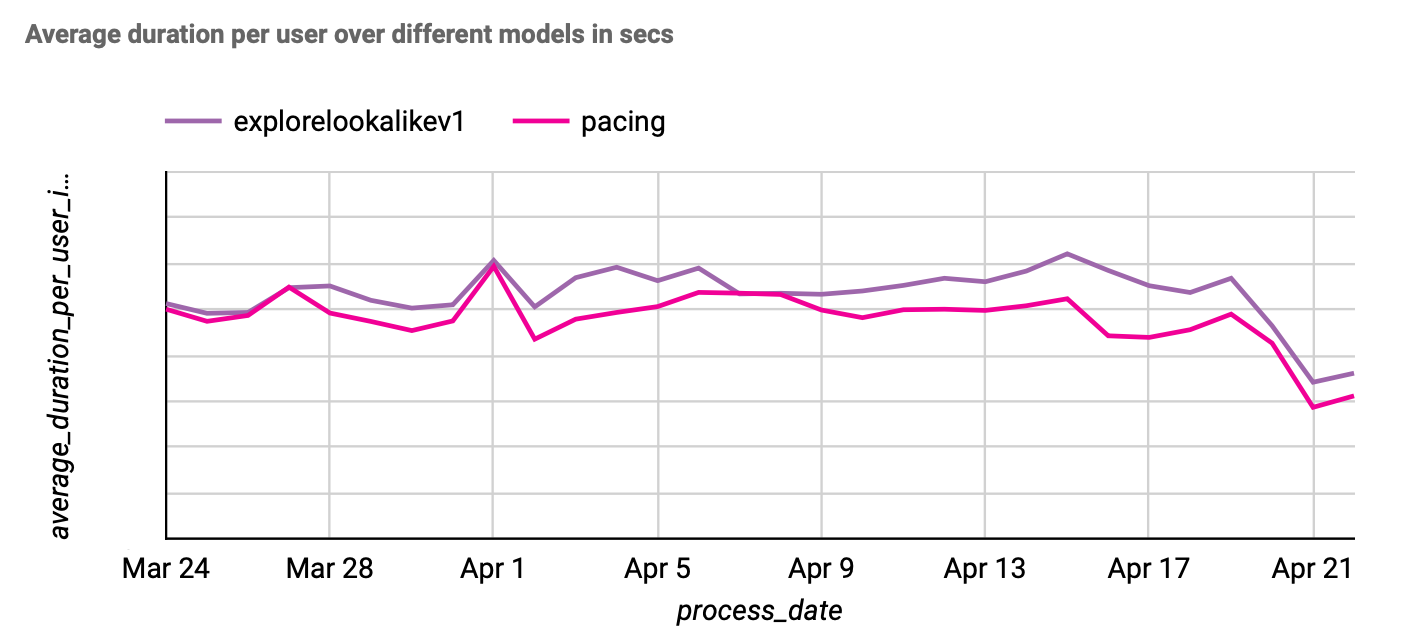
\includegraphics[width=\linewidth]{figures/DurationOverall-wrtPacing.png}
    \end{subfigure}%
    \begin{subfigure}
      \centering
      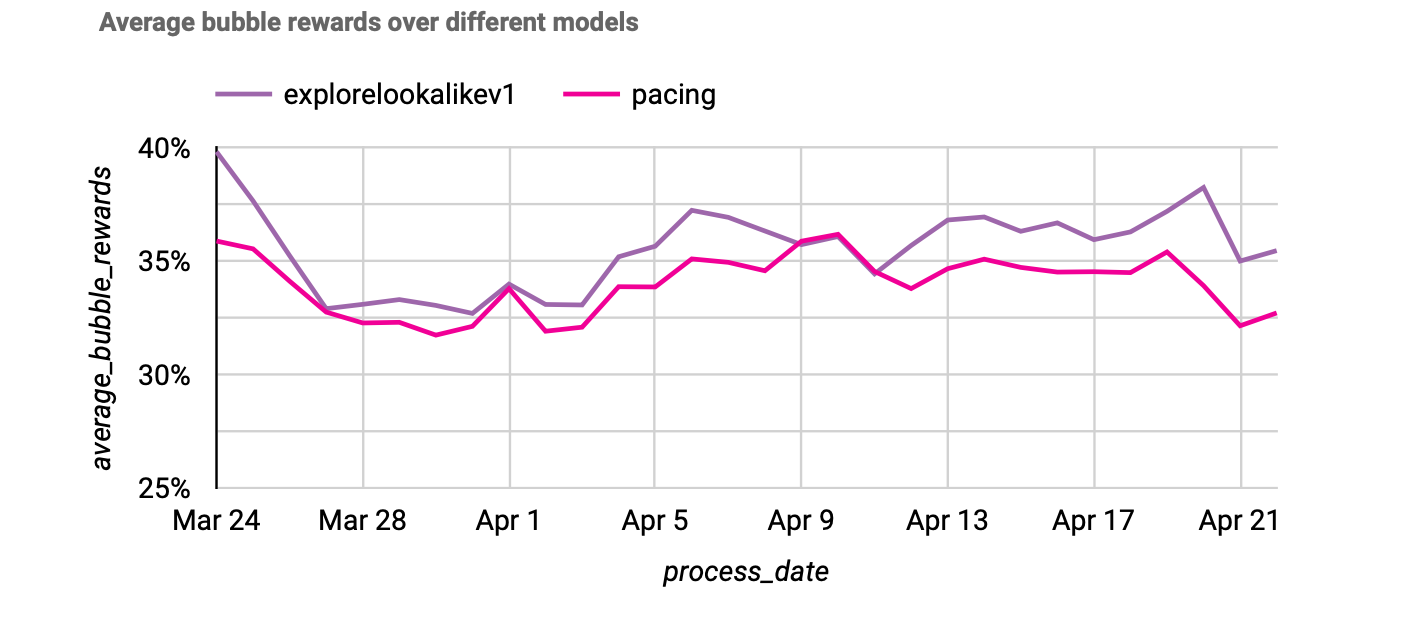
\includegraphics[width=\linewidth]{figures/BubRewardOverall-wrtPacing.png}
    \end{subfigure}
    \caption{Time spent (top) and Reward Rate (bottom) of our model as compared to Pacing, over all cohorts}
    \label{fig:comp_pacing_overall}
\end{figure}

When compared to the other models (Figure \ref{fig:comp_3_overall}) during the same period, our model routinely beats them on both the metrics, although by a smaller margin.  

\begin{figure}
    \centering
    \begin{subfigure}
      \centering
      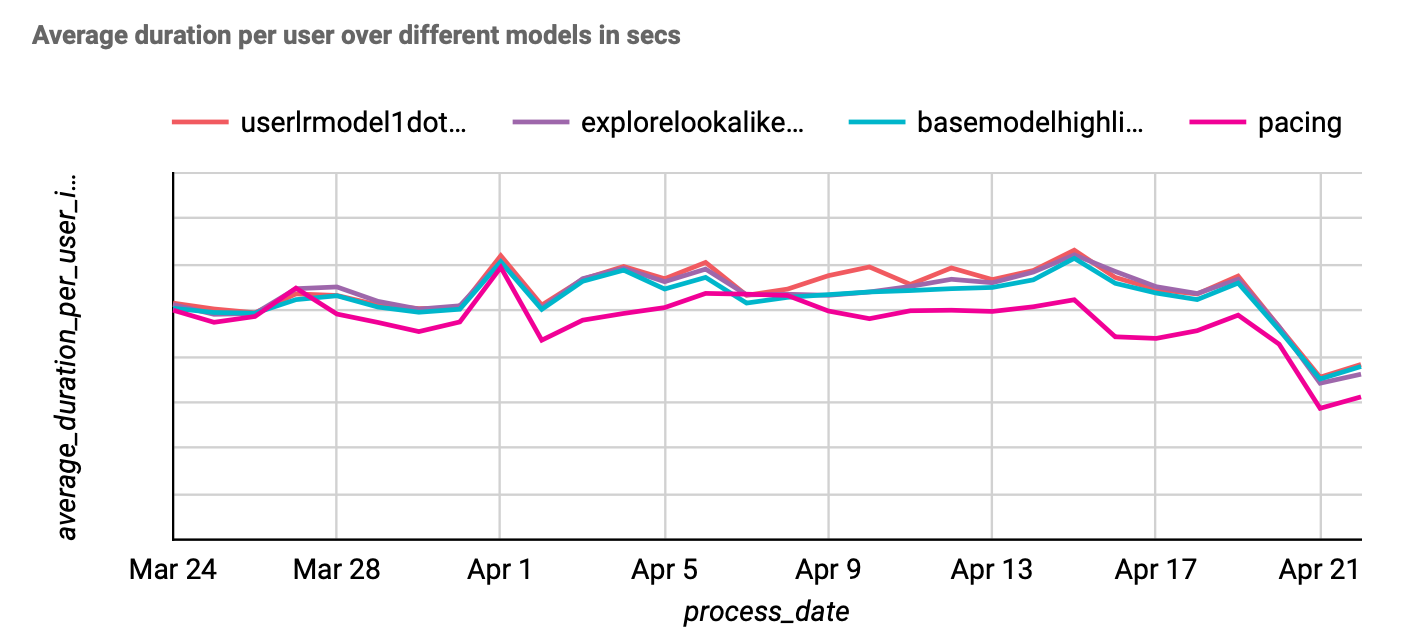
\includegraphics[width=\linewidth]{figures/DurationOverall-wrt3.png}
    \end{subfigure}%
    \begin{subfigure}
      \centering
      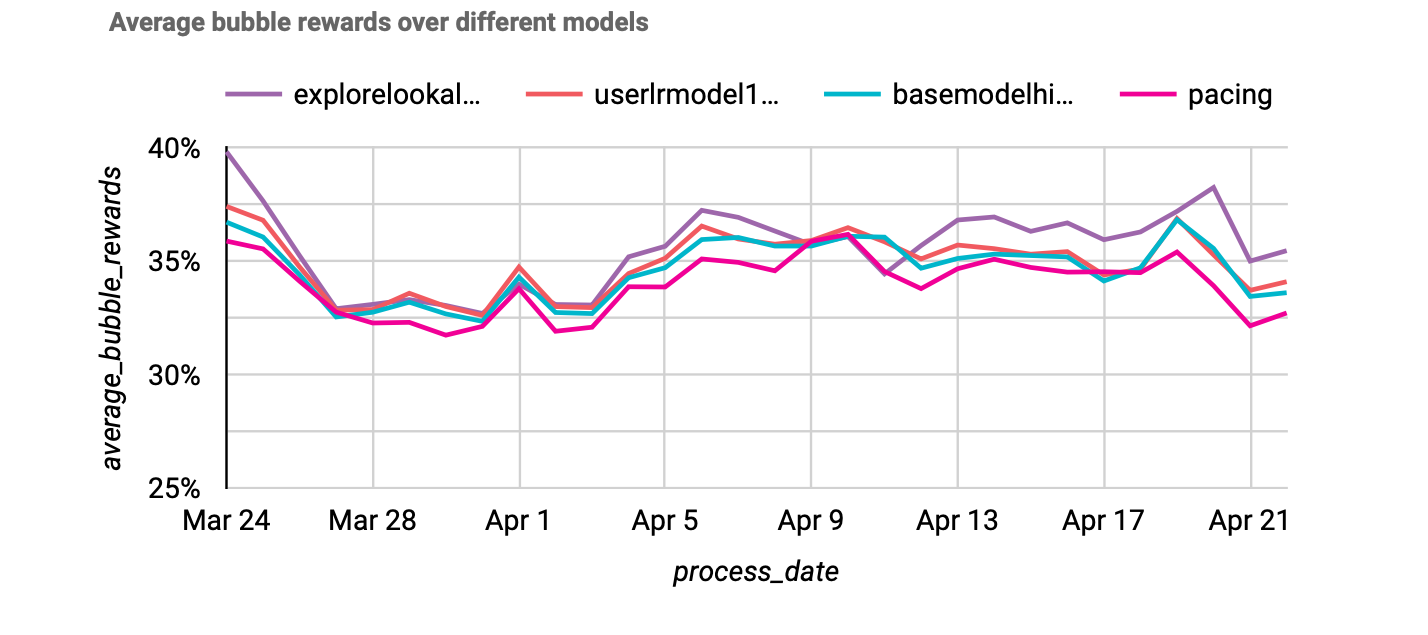
\includegraphics[width=\linewidth]{figures/BubRewardOverall-wrt3.png}
    \end{subfigure}
    \caption{Time spent (top) and Reward Rate (bottom) of our model as compared to other models, over all cohorts}
    \label{fig:comp_3_overall}
\end{figure}

Note that this across all the cohorts – cold, sparse, and dense. Because our model was trained on Dense users it was bound to perform well for them. It will not be sustainable, however, as at this stage it is only identifying popular content in specific categories for the users. If scaled it will not be able to explore content as well as a standard MAB. 

For Cold users (Figure \ref{fig:comp_pacing_cold}), the model performance comes out more distinctly. An average lift of 18.38\% in Time Spent and 5.76\% in Reward Rate as compared to Pacing. We also see competitive (and, at worst, at par) performance with respect to the other models (Figure \ref{fig:comp_3_cold}). 

\begin{figure}
    \centering
    \begin{subfigure}
      \centering
      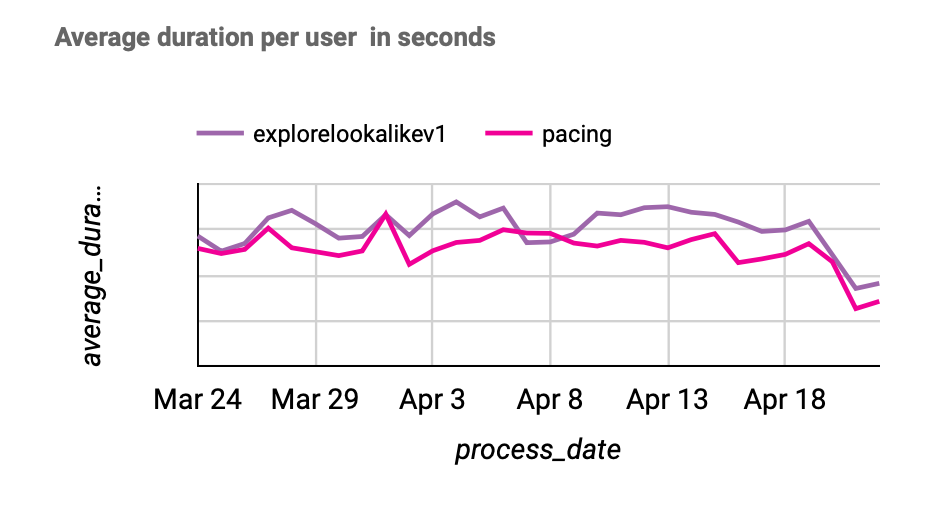
\includegraphics[width=\linewidth]{figures/DurationCold-wrtPacing.png}
    \end{subfigure}%
    \begin{subfigure}
      \centering
      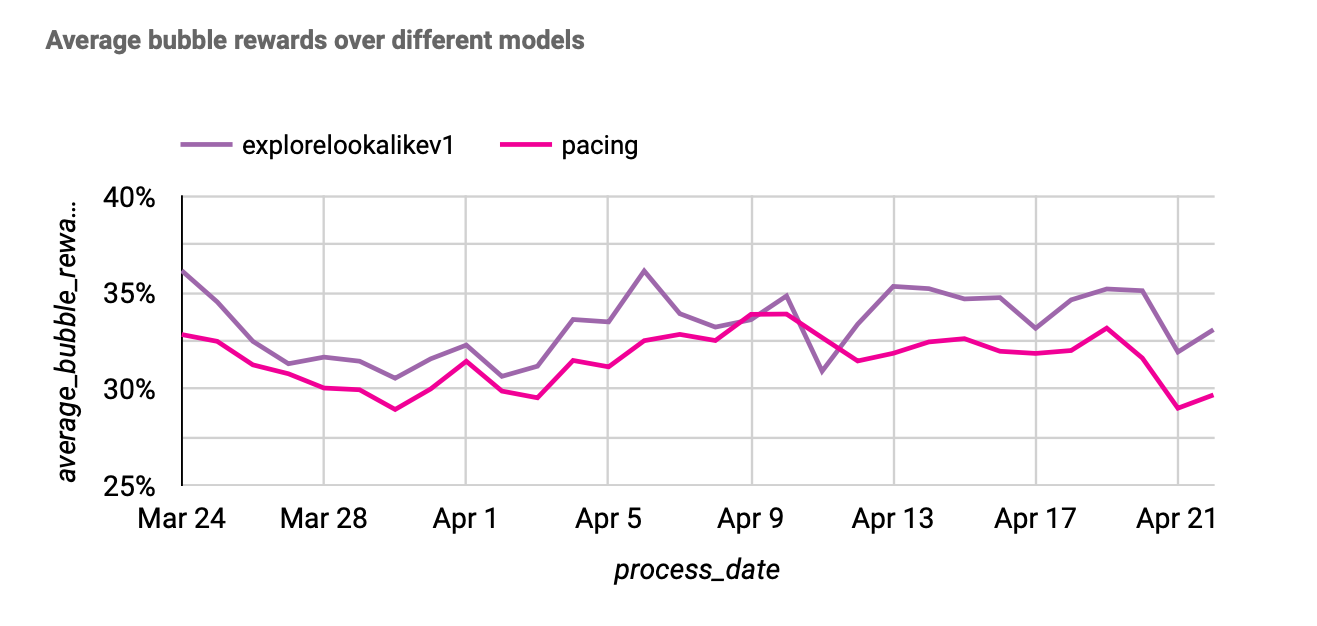
\includegraphics[width=\linewidth]{figures/BubRewardCold-wrtPacing.png}
    \end{subfigure}
    \caption{Time spent (top) and Reward Rate (bottom) of our model as compared to Pacing, for Cold Users}
    \label{fig:comp_pacing_cold}
\end{figure}

\begin{figure}
    \centering
    \begin{subfigure}
      \centering
      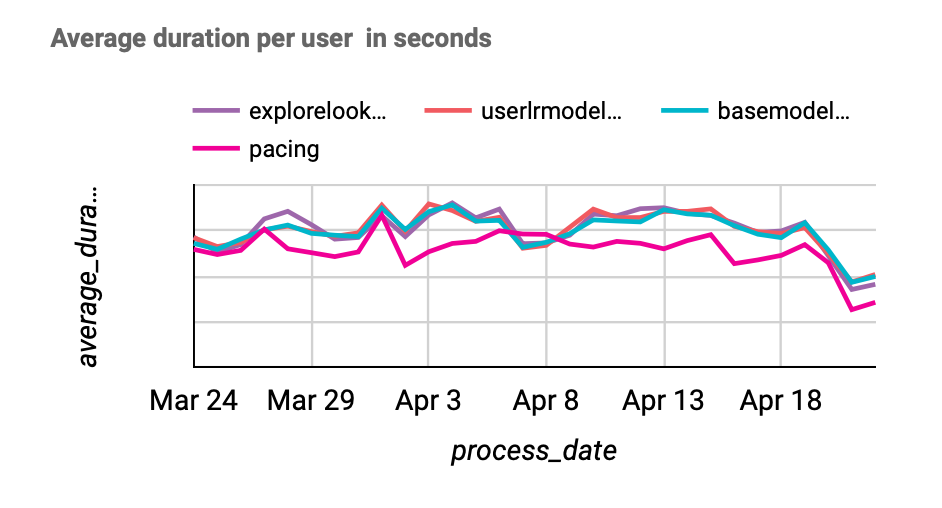
\includegraphics[width=\linewidth]{figures/DurationCold-wrt3.png}
    \end{subfigure}%
    \begin{subfigure}
      \centering
      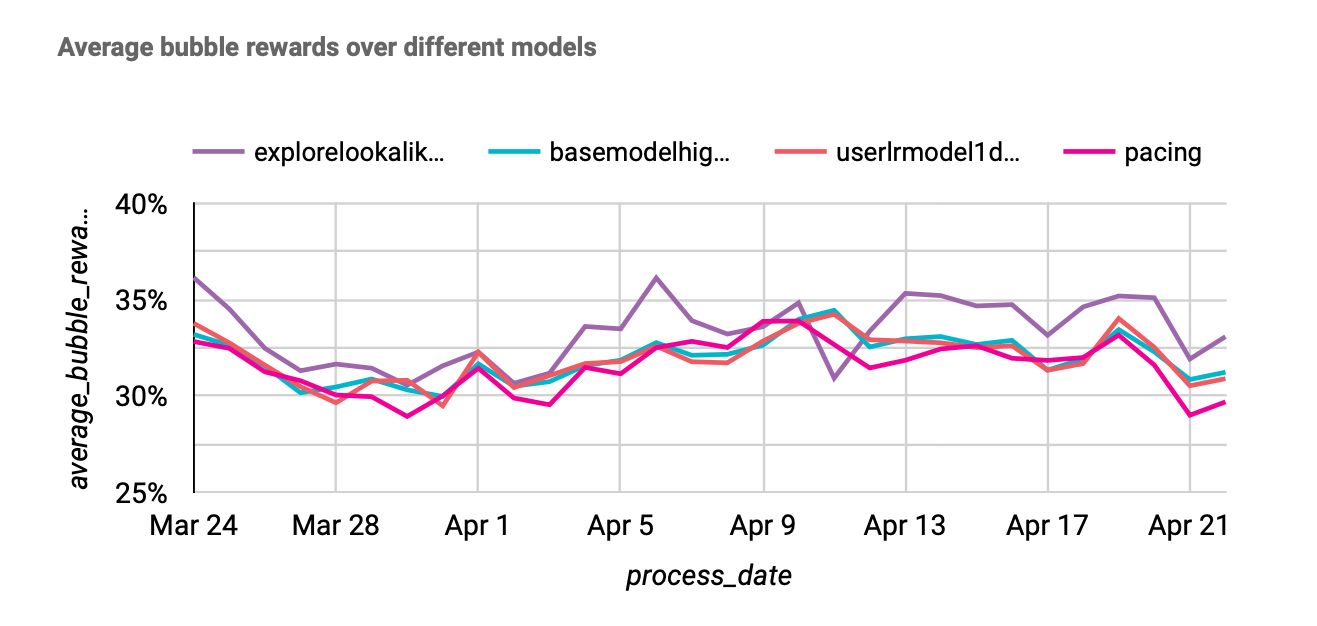
\includegraphics[width=\linewidth]{figures/BubRewardCold-wrt3.png}
    \end{subfigure}
    \caption{Time spent (top) and Reward Rate (bottom) of our model as compared to other models, for Cold Users}
    \label{fig:comp_3_cold}
\end{figure}

% \begin{figure*}
%     \centering
%     \begin{subfigure}
%       \centering
%       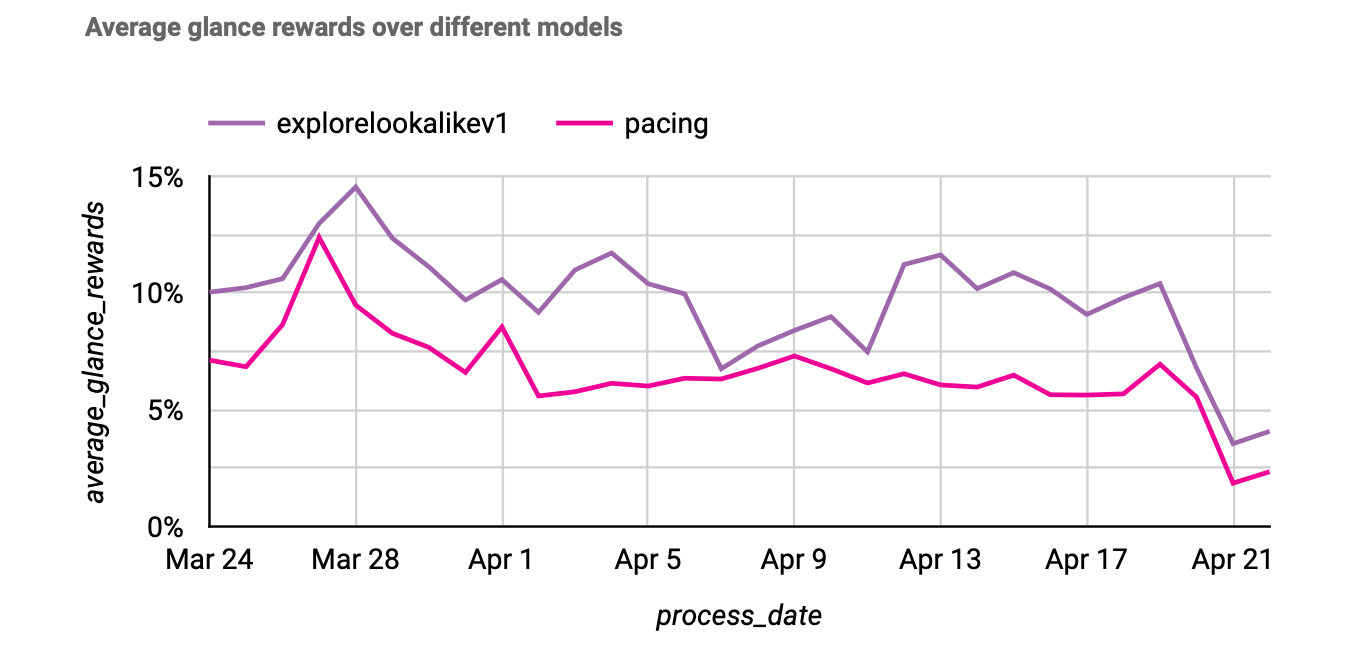
\includegraphics[width=0.45\textwidth]{figures/GlRewardCold-wrtPacing.png}
%     \end{subfigure}%
%     \begin{subfigure}
%       \centering
%       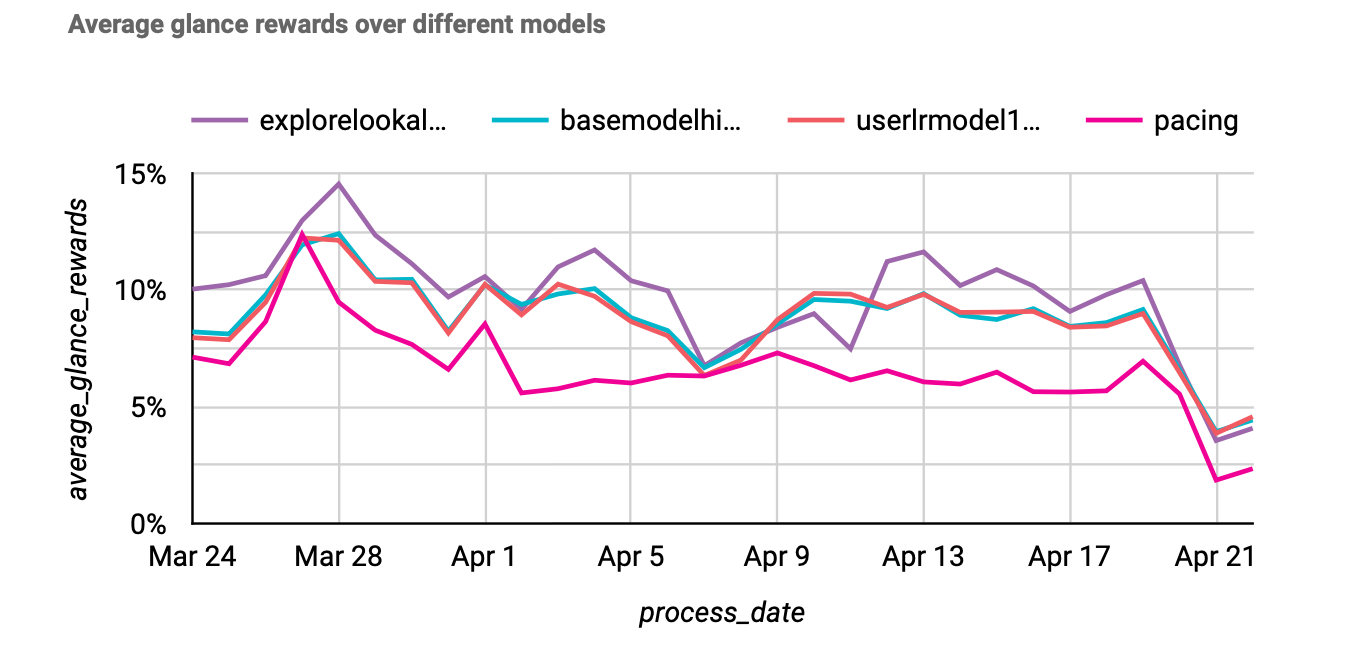
\includegraphics[width=0.45\textwidth]{figures/GlRewardCold-wrt3.png}
%     \end{subfigure}
%     \caption{Reward Rate at Glance level as compared to Pacing (left) and other models (right), for Cold Users}
%     \label{fig:comp_gl_reward}
% \end{figure*}

The improvement is especially stark when looked at the Reward Rate at Glance level, for Cold users (Figure \ref{fig:comp_gl_reward}. An average lift of 51.8\% as compared to Pacing and consistently beating out the other models. Our model, thus, performs well across all the metrics, especially so on Cold users.


